\documentclass[11pt, oneside]{article}   	% use "amsart" instead of "article" for AMSLaTeX format
\usepackage[margin=1 in]{geometry}                		% See geometry.pdf to learn the layout options. There are lots.
\geometry{letterpaper}                   		% ... or a4paper or a5paper or ... 
%\geometry{landscape}                		% Activate for rotated page geometry
%\usepackage[parfill]{parskip}    		% Activate to begin paragraphs with an empty line rather than an indent
\usepackage{graphicx}				% Use pdf, png, jpg, or eps§ with pdflatex; use eps in DVI mode
								% TeX will automatically convert eps --> pdf in pdflatex		
\usepackage{amssymb}

\usepackage{amsmath}

\usepackage{url}
\usepackage{hyperref}

\newtheorem{proposition}{Proposition}
\newtheorem{example}{Example}

\usepackage{listings}
%SetFonts

%SetFonts
\usepackage{xcolor}
\usepackage{float}

\title{\vspace{-.3 in} Investment Portfolios}
\author{Nick Arnosti}
\date{August 6, 2018}							% Activate to display a given date or no date

\begin{document}
\maketitle
%\section{}
%\subsection{}


\section{Motivation}

A common piece of investing advice goes as follows:\footnote{Quote taken from {\color{blue} \tt{\href{https://www.fool.com/retirement/2016/07/04/why-vanguard-target-date-funds-are-the-best-in-the.aspx}{\underline{the Motley Fool}}}}.}

\begin{quote}
\it Stock-based funds have higher long-term return potential but also have relatively high volatility. On the other hand, bond funds are more stable, especially in terms of income, but don't have the long-term growth potential of stocks. Therefore, it's generally suggested that younger investors put most of their money into stocks and gradually shift their investments into bonds as they get closer to retirement.
\end{quote} %Stocks are riskier than bonds, but have a higher expected return. Therefore, investors with long time horizons should invest primarily in stocks, and those nearing retirement should invest primarily in bonds.


For investors that don't want to actively manage their retirement portfolio, companies such as Vanguard have introduced ``Target Date Funds" (TDFs), which are marketed as a ``one stop shop" for retirement investing. {\color{blue} \tt{\href{https://investor.vanguard.com/mutual-funds/target-retirement/#/}{\underline{Vanguard's explanation}}}} states,  ``managers gradually shift each fund's asset allocation to fewer stocks and more bonds so the fund becomes more conservative the closer you get to retirement" (see Figure \ref{fig:glidepath}). 
%This approach is depicted in Figure \ref{fig:glidepath}, taken from the US department of labor's {\color{blue} \tt \href{https://www.dol.gov/sites/default/files/ebsa/about-ebsa/our-activities/resource-center/fact-sheets/investor-bulletin-target-date-retirement-funds.pdf}{\underline{investment bulletin}}} on TDFs. 
My employer plan goes straight to a TDF, and I am not alone: according to this {\color{blue} \tt \href{https://www.forbes.com/sites/markavallone/2018/06/30/why-target-date-funds-dominate-the-401k-market/#8081c8758687}{\underline{Forbes article}}}, most employer-sponsored retirement funds default to TDFs, and it is predicted that 88\% of retirement plan contributions will flow into TDFs by 2019.

TDFs are popular, but does their approach actually make sense? In this post, I investigate that question, taking as given the assertion that stocks are riskier than bonds, but have a higher expected return. I start by introducing a simple model that will frame my thinking, present cases against and for shifting assets from stocks to bonds over time, and close with an informal discussion.


\begin{figure}[!h]
\centerline{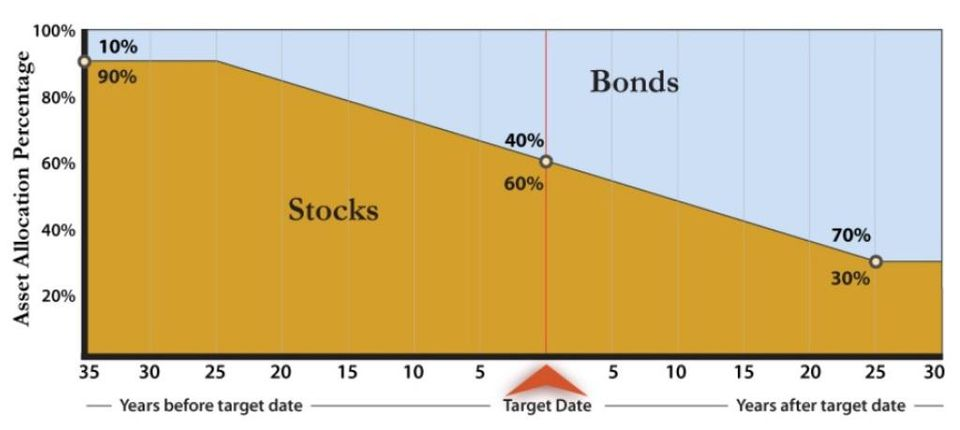
\includegraphics[width = 0.8\textwidth]{Glidepath-Sample-1}}
\caption{Mix of stocks and bonds in a Target Date Fund over time. Source: US Department of Labor {\color{blue} \tt \href{https://www.dol.gov/sites/default/files/ebsa/about-ebsa/our-activities/resource-center/fact-sheets/investor-bulletin-target-date-retirement-funds.pdf}{\underline{investment bulletin}}} on TDFs.}
\label{fig:glidepath}
\end{figure}

\newpage

\section{Model}
An investor starts with \$1. In each period $t$, she may place a fraction $\alpha_t$ of her wealth in a risky asset, with (unknown) return $r_t$; the remaining $1 - \alpha_t$ fraction of her wealth goes into a safe asset with known return $s$. Given returns $r_t$ and investment decisions $\alpha_t$, her per-period wealth $W_t$ evolves as follows:

\[W_{t+1} = (\alpha_t r_t + (1 - \alpha_t) s) W_t.\]

Assume that $s \geq 1$ and $r_t$ are iid draws from a known distribution $G$, with $E[r_t] > s$ and $P(r_t < s) > 0$. Our investor plans to retire in period $T$. Her final utility is given by $U(W_T)$ for some known and weakly increasing function $U$, and she invests to maximize her expected utility.

%Candidates:
%\begin{enumerate}
%\item $U(x) = x$
%\item $U(x) = \log(x)$. Captures risk aversion.
%\item $U(x) = {\bf 1}(x \geq w)$. Captures target.
%\item $U(x) = (1 + e^{-\lambda (x-w)})^{-1}$. Captures idea that if you're poor, things don't get too much worse, and if you are rich, there is little (though some) value to more money.
%\end{enumerate}
%To me, the most plausible cases are 2 and 4 above.

\section{The Contrarian}

I start by presenting evidence {\em against} the conventional wisdom that investors should gradually shift from stocks to bonds. 

\begin{proposition}
If investors maximize expected wealth $(U(x) = x)$, then it is optimal to select $\alpha_t = 1$ for all $t$.
\end{proposition}

Of course, most investors don't aim to maximize expected wealth. Generally, money is assumed to have diminishing marginal returns. One standard assumption that captures this effect is to take $U(x) = \log(x)$, implying that in order to increase the utility of two different investors by equal amounts, it is necessary to increase their wealth by equal {\em percentages}. In this case, it may make sense to invest in a mix of bonds and stocks, but the optimal mix does not depend on one's wealth level or the time until retirement.

%a 10\% increase in wealth increases the utility of agents at different wealth levels by an equal amount.

\begin{proposition}
If investors maximize the expected logarithm of wealth $(U(x) = \log(x))$, then there exists $\alpha \in [0,1]$ such that it is optimal to select $\alpha_t = \alpha$ for all $t$. 
\end{proposition}

%Note that under these conditions, the optimal investment portfolio is constant in $t$, independent of $T$, static (doesn't depend on past luck), and independent of wealth level. 

Of course, $U(x) = \log(x)$ is still one particular functional form. However, it turns out that for {\em any} utility function $U$, committing to any particular trajectory of the stock-bond mix is no better than committing to the reverse.

%Suppose that you don't believe that $U(x) = \log(x)$ is the right functional form. 

\begin{proposition} \label{prop:static}
If investors follow a non-adaptive policy\footnote{I say that a policy is non-adaptive if $\alpha_t$ is independent of the vector of returns ${\bf r}$.} $\alpha = (\alpha_1, \ldots, \alpha_{T-1})$, then the distribution of $W_T$ is invariant to a permutation in $\alpha$.
\end{proposition}

\newpage

\section{Adaptive Investment}

Proposition \ref{prop:static} establishes that among non-adaptive investment policies, there is no reason that the investment in stocks should decrease over time. However, in practice investors can use adaptive policies. For example, I might shift my money to bonds if I know I have enough to retire on, but keep it in stocks if I had bad initial luck and need to hope for big returns in the future. 

Given any utility function $U$ and distribution of returns $G$, it is possible to use dynamic programming to solve for the optimal adaptive policy (as a function of the current wealth level and time until retirement). The results are given in Figure \ref{fig:alpha}. (Code provided in Section \ref{sec:code} -- no apologies for its limitations, as one of the joys of being an academic is being able to write non-robust code.)

\begin{figure} 
\centerline{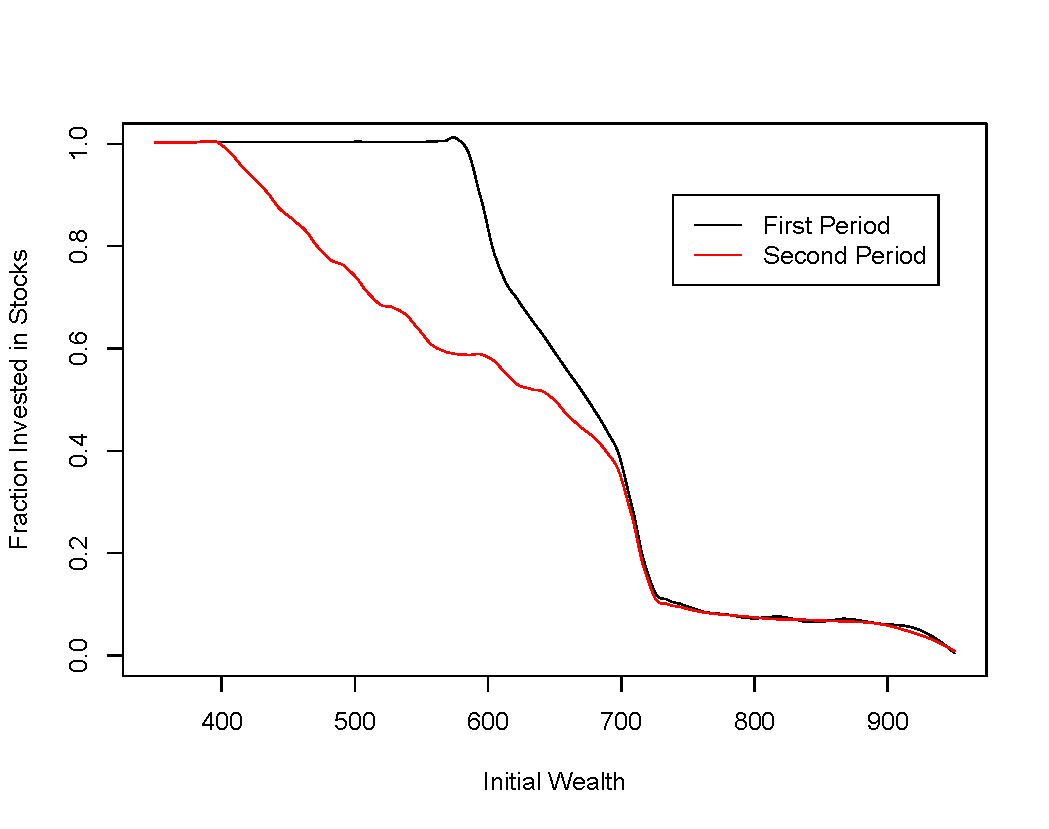
\includegraphics[width=.5\textwidth]{InvestmentAdvicePlot.pdf}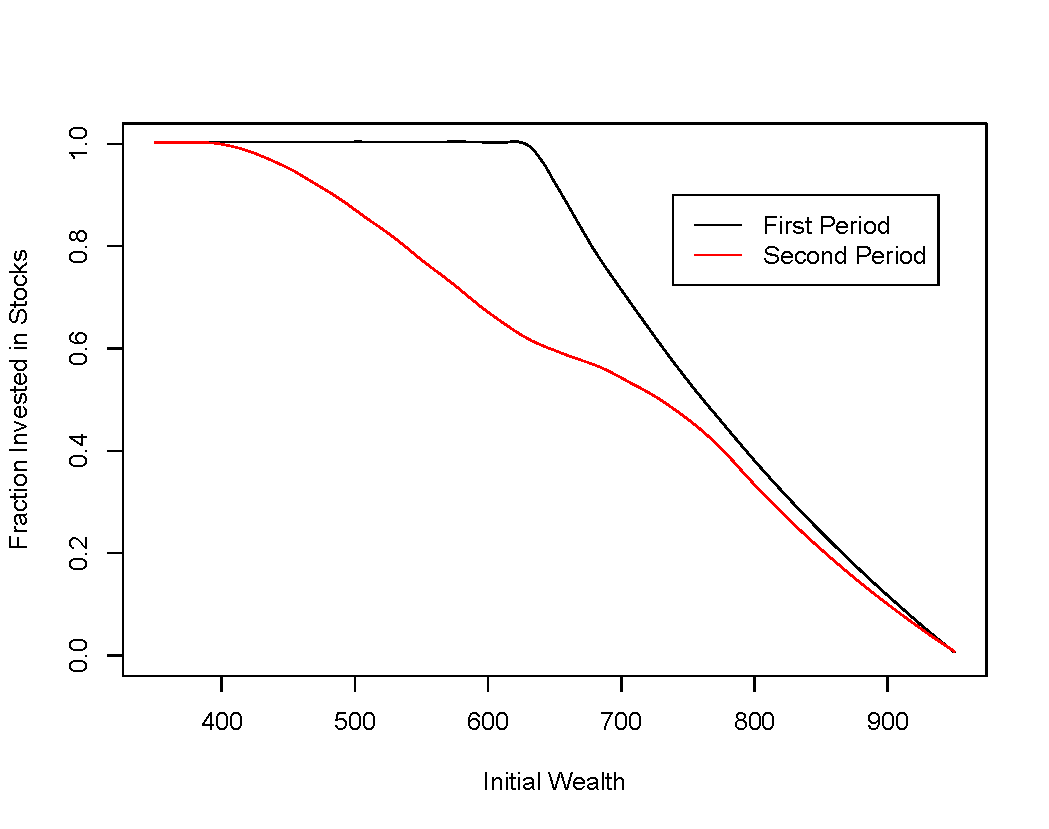
\includegraphics[width=.5\textwidth]{InvestmentAdvicePlot2.pdf}}
\caption{Average percentage of portfolio invested in stocks under optimal policy, as a function of initial wealth. Left side is $U(x) =  (1+e^{-(x-b)/50})^{-1}$, right side is $U(x) = \frac{1}{2} \sqrt{x/650}.$ }
\label{fig:alpha}
\end{figure}
%there is no reason to commit to gradually decreasing the percentage of the portfolio invested in stocks: one would do just as well to start with mostly bonds, and gradually shift to more stocks.

%committing to gradually decreasing the percentage of the portfolio invested in stocks is no better than committing to gradually increasing the 




My intuition for these  plots is that the desire to {\em acquire information} about returns encourages the investor to front-load her investment in stocks. This is illustrated by the simple example below.\footnote{I would be curious establish conditions under which the investor expects to hold a higher percentage of stocks in the first period than the second. One tricky aspect is that while the value function is unique, the optimal policy may not be. I know that there sometimes exist optimal strategies under which the expected fraction of the portfolio invested in stocks increases over time, but it is conceivable to me that there always exists an optimal strategy under which the investor expects to gradually shift to bonds.} 
% there is value to {\em learning about my luck earlier}, so that I can adjust my investment decisions accordingly. Consider an investor who has a target 

\begin{example}
Suppose that $s = 1.1$ and $r \in \{L, M, H\}$, with $L = 0.8, M = 1.2, H = 1.65$. Let $p_L = P(r_t = L)$, and similarly for $p_M$ and $p_H$. Suppose that an investor has $\$500,000$ in savings, is two years from retirement, and wants to retire with at least $\$650,000:  U(w) = {\bf 1}(w \geq \$650,000)$.

Let us first consider non-adaptive strategies. The investor cannot invest in safe assets alone, as she will not reach her retirement goal. If she invests only in risky assets, she will succeed so long as neither period has low returns, or at least one period has high returns. Her chance of success is $1 - p_L(p_L + 2p_M)$. If she invests in safe assets in the first period, and risky assets in the second, she will succeed whenever the return in the second period is not $L$. Her success probability is $1 - p_L$. 

An optimal strategy is adaptive. By investing in risky assets in the first period, the investor gains information. If her initial return is $M$ or $H$, she can lock her wealth in safe assets during the second period; if her initial return is $L$, she knows that she must invest in risky assets in the second period, hoping for a high return. Her probability of success under this strategy is $1 - p_L(p_L + p_M)$, and on average her portfolio has more safe assets in the second period.
\end{example}


\section{Discussion}

So, does the conventional wisdom make sense? My answer is a qualified yes. An investor who actively manages her portfolio to prepare for retirement might reasonably expect to see the percentage of stocks decline over the years. The reason for this is that investing in stocks early {\em provides information} which can be used to make future decisions\footnote{In the model, the only decision is the mix of stocks and bonds, but in reality an investor may also choose to change consumption behavior before retirement or work for a few extra years.} -- if this information is not used, then there is no reason to gradually shift the portfolio from stocks to bonds.

This suggests that sales pitch for Target Date Funds (TDFs) doesn't really make sense -- they cater to investors who want to set aside money and forget about it until retirement, but adopt a ``glide" strategy that can't easily be justified for these investors. 

As one {\color{blue} \tt \href{https://www.investopedia.com/articles/retirement/07/life_cycle.asp#ixzz5NBlgpyaP}{\underline{Investopedia article}}} states,
\begin{quote}
\it One retiree may have enough money on hand to invest strictly in bonds and other fixed-income securities. Another, requiring both growth and income, may need an equity component to keep the portfolio on track. A fund that meets the needs of one of these investors is unlikely to meet the needs of the other.
\end{quote}

Will I redirect my contributions away from the Target Date Fund? Not right away -- it's mostly stocks right now, as it likely should be. But don't be surprised if I end up shifting the money more actively at some point in the future.

%If an investor wants to simply ``set aside money and forget about it until retirement", 


%Clearly, this assumes something about risk preferences -- if investors maximize expected welfare, they should go all stocks, all the time. Obviously, if I have plenty of money at the end of life, I don't want to spin the roulette wheel by putting it in stocks. But if I am approaching retirement and don't have enough to live on, I may want to do just that! Conversely, even if I am young, if I know how much I need to retire and can earn that much by investing only in bonds, why do I need stocks?
%
%
%My guess: none of the three utility specifications below lead to the conventional wisdom for {\em any} investor (any time horizon $T$ and utility function $U$). What specifications, if any, justify this advice?
%
%Among static portfolios, note that distribution of $W_T$ is invariant to permutations of $\alpha$. In other words, investing mostly in stocks for 10 years at the beginning and mostly in bonds for 10 years at the end leads to the same distribution of possible outcomes as doing the reverse -- so for any utility function (that depends only on $W_T$), it can't be better to do the former.

%compare one that initially invests $\alpha_H$, and later invests $\alpha_L$, to one that invests $\alpha_M \in (\alpha_L, \alpha_H)$. Intuitively, the former is more risky -- if initial returns are bad, we will be set way back!

\section{Code} \label{sec:code}

{\footnotesize
\begin{lstlisting}[language=R]
#Given vectors X,Y such that X is increasing and Y = g(X), 
#returns a discretized function approximating g
approximate = function(X,Y){
	return(Vectorize(function(x){
		i = max(c(which(X < x),1))
 		return(Y[i]) #Could do linear interpolation, but why bother?
	}))
}

#Given current wealth w, return from safe and risky assets, and value function V, 
#computes expected utility from any given alpha
#Assumes p is probability vector of the same length as r, and s and w are scalars
expectedUtility = function(w,s,r,p,V){
 	return(Vectorize(function(alpha){
 		 return(sum(V((alpha*r+(1-alpha)*s)*w)*p))
 	}))	
}


s = 1  #return from safe asset
r = .6 + c(0:10)/10  #possible returns from risky asset
p = rep(1/length(r),length(r)) #p[i] is probability of return r[i]

a = 0.02; b= 650;
N = 250
W = b+6*rep(-N:N)/(a*N)   #Different levels of wealth, in a range relevant to U


#U for plot 1
U = Vectorize(function(x){return(1/(1+exp(-a*(x-b))))})   

#U for plot 2
U = Vectorize(function(x){return(sqrt(x/b)/2)})

#Target of 650
#U = Vectorize(function(x){if(x>=650) return(1); return(0)})

T = 2

#V[t+1,i] gives value of having W[i] dollars with t periods remaining
V = matrix(0,nrow = T+1,ncol=length(W)) 
#Alpha[t+1,i] gives optimal portfolio wit W[i] dollars and t periods remaining
Alpha = matrix(0,nrow = T+1,ncol=length(W)) 
V[1,] = U(W)
for(t in 1:T){
	for(i in 1:length(W)){
		#soln = optimize(expectedUtility(W[i],s,r,p,approximate(W,V[t,])),interval=c(0,1),maximum=TRUE)
		#Alpha[t+1,i] = soln$maximum  #Optimal alpha, given t remaining periods and wealth level W[i]?
		#V[t+1,i] = soln$objective #Expected value, given t remaining periods and wealth level W[i]?
		
		#Optimize function works poorly for locally flat functions,
		#so taking this approach instead
		EU = expectedUtility(W[i],s,r,p,approximate(W,V[t,]))(c(0:N)/N)  
		V[t+1,i] = max(EU)  
		Alpha[t+1,i] = which(EU==max(EU))[1]/N
	}
}
#filled.contour(V,x = c(0:T),y=W,xlab='Time Remaining',ylab='Wealth')


#Two period model -- compare alpha in first period to average alpha in second period
AlphaSecondPdAvg = rep(0,length(W))  #AlphaSecondPdAvg[i] gives average alpha in second period, when investor has W[i] with two periods to go and behaves optimally
alphafn = approximate(W,Alpha[2,])  #alphafn(w) says what alpha to choose, given wealth of w and one period remaining
for(i in 1:length(W)){
	AlphaSecondPdAvg[i] = sum(alphafn((Alpha[3,i]*r+(1-Alpha[3,i])*s)*W[i])*p)  #Alpha[3,i] is optimal alpha, given wealth W[i] with two periods remaining
}

plot(NULL,xlab='Initial Wealth',xlim=c(W[1],W[length(W)]),ylab='Fraction Invested in Stocks',ylim=c(0,1))
lines(W,predict(loess(Alpha[3,]~W,span=0.1)),col='black')
lines(W,predict(loess(AlphaSecondPdAvg~W,span=0.1)),col='red')
legend(x=W[N*1.3],y=0.9,legend = c('First Period','Second Period'),col=c('black','red'),lty=c(1,1))


\end{lstlisting}

}

\end{document}  